\documentclass{standalone}
\usepackage{tkz-base}
\usepackage{tkz-fct}
\usepackage{tkz-euclide}
\usepackage{tikz}
\begin{document}
    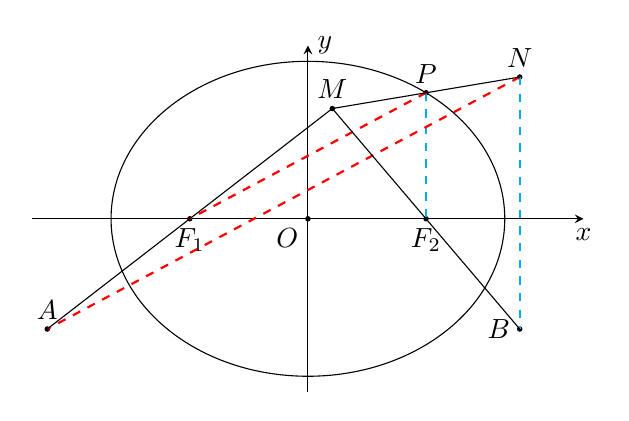
\begin{tikzpicture}
        \pgfmathsetmacro\x{3.5}
        \pgfmathsetmacro\y{2.2}
        \pgfmathsetmacro\a{2.5}
        \pgfmathsetmacro\b{2}
        \pgfmathsetmacro\c{sqrt(abs(\a^2-\b^2))}
        \pgfmathsetmacro\px{1.5}
        \pgfmathsetmacro\py{sqrt((\b^2)*(1-((\px)^2)/(\a^2)))}
        \coordinate (O) at (0,0);
        \coordinate (F1) at (-\c,0);
        \coordinate (F2) at (\c,0);
        \coordinate (P) at (\px,\py);
        \coordinate (E) at ($(P)!0.5!(F1)$);
        \coordinate (M) at (0.31,1.4);
        \coordinate (A) at ($(M)!2!(F1)$);
        \coordinate (B) at ($(M)!2!(F2)$);
        \coordinate (N) at ($(M)!2!(P)$);
        \draw[-stealth] (-\x,0) -- (\x,0) node [below] {$x$};
        \draw[-stealth] (0,-\y) -- (0,\y) node [right] {$y$};
        \fill (O) node [below left] {$O$} circle (1pt);
        \fill (F1) node [below] {$F_1$} circle (1pt);
        \fill (F2) node [below] {$F_2$} circle (1pt);
        \fill (P) node [above] {$P$} circle (1pt);
        \fill (A) node [above] {$A$} circle (1pt);
        \fill (B) node [left] {$B$} circle (1pt);
        \fill (N) node [above] {$N$} circle (1pt);
        \fill (M) node [above] {$M$} circle (1pt);

        \draw (O) circle [x radius=\a,y radius=\b];
        \draw[cyan,dashed,thick] (N)--(B) (P)--(F2);
        \draw[red,dashed,thick] (N)--(A) (P)--(F1);
        \draw (A)--(M)--(B) (M)--(N);
    \end{tikzpicture}
\end{document}